\section{Design}\label{design}

This section describes the design process that was followed to create the application featured in this thesis. First, we propose a solution for several issues highlighted in the literature review. Based on the proposal, additional literature was reviewed to guide the design of the prototype. Section~\ref{guiding_principles} describes these guiding principles. The first step of the design process led to the creation of several personas and scenarios, found in section~\ref{personas_scenarios}. Hereafter, we define the functionality of the prototype with the help of a small brainstorm session. To conclude, a concrete specification and mockups of the prototype are given.

    % we provide arguments
    \subsection{Proposal}
    
    The literature review indicated that several issues arose after EHR systems were installed. In this section we gather those issues and propose a solution that remedies them. During the definition of our solution, arguments are given as to why certain choices are made.

    \paragraph{Current issues} In some cases, the use of an EHR led to an increase in medical errors. Research showed that poor usability was one of the causes for this rise~\cite{Koppel2005}. Another study found that the use of paper workarounds was also responsible for this increase~\cite{Saleem2009}, which again hints at a system with poor usability. However, the use of these workarounds also indicates that the system is not in line with the workflow of the clinician.

    The installation of a new EHR system disrupts the current workflow significantly~\cite{Menachemi2011}. Large updates to an existing system may also cause disruptions. Clinicians need to be trained in order to work efficiently with the new system. If there is insufficient training, more medical errors may occur. It takes some to become accustomed to these changes, which leads to a temporary loss of productivity. Sometimes this adaptation process is difficult for some individuals which may spark negative emotions.

    \paragraph{Solution} We propose a EHR web application featuring at its core a customizable dashboard. The clinician may freely place and arrange modules on the dashboard, similar to placing widgets on the homescreen found within the Android OS\@. Behind-the-scenes, creating new modules for the dashboard should be a straightforward process. In terms of usability, the modules share a clear and concise design, and the dashboard can adapt to different screen sizes. We now go into more detail.

    The choice of creating a web application was quickly made, since these applications are cross-platform out of the box. Updating the application is done by simply refreshing the web page. The development and extension of native applications for several operating systems is very costly as multiple teams of developers are needed. Also, recent web technology advancements allow much more complex applications to be run straight from the browser. To give an example, Microsoft provides a web app version of its Office Suite. 

    The dashboard presents a novel approach regarding interoperability. Instead of providing interoperability for multiple standalone applications, the dashboard is continuously expanded with new modules. In other words, applications are integrated as new modules of the dashboard. This module-based approach has several benefits:
    \begin{itemize}
        \item There is no need to switch between multiple standalone applications, which may have completely different designs.
        \item Clinicians only need to learn to use the modules that are required for their workflow, instead of a complete software package.
        \item Many different workflows can be supported by using a combination of modules.
        \item The dashboard can easily adapt to workflow changes by allowing the addition and removal of modules.
        \item Module updates do not affect other modules or the dashboard, preventing total workflow disruption.
        \item Free placement of modules on a grid allows the dashboard to support many different screen sizes.
    \end{itemize}

    \noindent To guarantee a streamlined user experience throughout the dashboard, new modules inherit a template which determines its appearance. Changing this template, will change the appearance of all the modules. Also, dashboard will be designed with touch technology in mind to prevent usability issues such as the fat-finger problem and screen clutter. 
 
    In practice, vendors develop modules according to guidelines defined by the dashboard application. Integrating new modules to the dashboard still requires some work from the institution's IT staff, but no where near as much when integrating a standalone application. Once the module is integrated, it can be seamlessly updated. The dashboard also has the ability to import patient data.\bigskip

    \noindent In the end, the dashboard application features cross-platform availability, easy extension of functionality, a usable and customizable interface, and a simple learning process. At this stage, additional literature was consulted to facilitate the creation of an effective design.

    \subsection{Guiding principles}\label{guiding_principles}

    The translation of the aforementioned proposal to an intuitive prototype is guided by several principles. It was paramount during the design and implementation phases that the final prototype provided a positive user experience. This final prototype is the result of a series of steps defined by the MuiCSer framework, which is explained first. Hereafter, several design principles are mentioned that serve as helpful guidelines during the design process of a dashboard application.

        \subsubsection{MuiCSer}\label{muicser}
        % description of process
        This section describes the MuiCSer framework, designed for user-centered software engineering processes in a multidisciplinary context~\cite{Haesen2008}. This framework focuses on optimizing the user experience during the entire software engineering cycle to ensure that the needs of the end user are fulfilled. By combining user-centered design methodologies and software engineering principles, the user experience of the final product can be improved substantially. Given the multidisciplinary context of this thesis, MuiCSer guided the entire development process leading to the final prototype described in section~\ref{implementation}.
        
        \begin{figure}[!t]
            \centering
            
\includegraphics[width=0.8\textwidth]{chapters/3_design/muicser}
            \caption{The MuiCSer process.}\label{fig:muicser}
        \end{figure}

        The MuiCSer process is summarized in figure~\ref{fig:muicser}. After each phase, the result is evaluated, verified and validated to ensure that the required functionality is present. In turn, the received feedback can be used to reiterate over the previous phase. On the figure, this is denoted with the light blue arrows, while the single dark arrow represents the overall direction of the process. What follows is a brief description of each phase:

        \paragraph{1. New or legacy system} The MuiCSer process starts with either an existing system in need of improvement, or with a new system which needs to be built from the ground up. This requires an analysis of the tasks and needs of the user, as well as the objects and resources required to perform these tasks. Personas and scenarios are the resulting artifacts of this phase. First, personas describe the personalities of the potential end users including hobbies, skills and the environment they surround themselves in~\cite{Madsen2010}. Its goal is to uncover behavior patterns which can be of use when designing a user interface. Second, scenarios tell stories describing the use of a fictitious system from the point of view of a persona~\cite{Madsen2010}. To summarize, personas and scenarios try to sketch the usage of the system for which a design must be made. These artifacts are found in section~\ref{personas_scenarios}.

        \paragraph{2. Structured interaction analysis} During this phase, the results of the analysis are used to create task models. These models specify concrete tasks and goals which can be dissected into specific actions or steps the user has to take. These artifacts lay the foundation for designing a user interface which supports these tasks and goals. Task models were not created. Instead, via a brainstorm session (section~\ref{module_brainstorm}), common tasks of a health system were grouped to form modules. The user interface will be designed to support these modules.

        \paragraph{3. Low fidelity prototyping} After the task definition, low fidelity prototypes are created. Paper sketches and mockups are examples of low fidelity prototypes. Without spending too much time and resources, presenting these prototypes to the end-user or customer can yield valuable feedback. However, there is often no functionality present. Typically multiple versions of these prototypes are created until the customer is satisfied, after which the development of a high fidelity prototype starts. Low fidelity prototypes were created for all modules defined during the brainstorm session and are found in section~\ref{app_specification}.

        \paragraph{4. High fidelity prototyping} The development of high fidelity prototypes requires a lot more effort compared to low fidelity prototypes, as they offer functionality closely resembling the final product. However, the end user can now test both the design \emph{and} the functionality. This yields much more meaningful feedback. Section~\ref{implementation} describes the development of the high fidelity prototype.

        \paragraph{5. Final user interface} When the latest iteration of the high fidelity prototype satisfies all user requirements, the final user interface can be created. The high fidelity prototype may serve as the starting point of the final product in order to save time and resources. As a final step, the task models are checked against the resulting interface to check if all required functionality is present. No final product was created during the period of this thesis. However, the results of the usability test described in section~\ref{discussion} should determine if it is feasible to commit further research towards the prototype.

        \subsubsection{Dashboard design}\label{dashboards}

        The proposal mentions a dashboard. However, dashboards are used in many contexts. Common examples include a car speedometer and stock analysis. In computer networking, dashboards are used to quickly interpret network traffic. In our case, we want to empower the user to create his or her own dashboard. To facilitate this goal, several design principles should be kept in mind.
        
        While some dashboards provide fancy graphics, many miss the key point of what they are supposed to accomplish. The primary goal of a dashboard is clear communication, which is achieved through effective design. A formal definition is as follows: ``A dashboard is a visual display of the most important information need to achieve one or more objectives; consolidated and arranged on a single screen so information can be monitored at a glance.''~\cite{Few2006}. This definition contains four key characteristics:

        \paragraph{Dashboards are visual displays.} It is important that data is represented visually. Graphics such as charts allow more efficient communication compared to textual information. For example, trends and outliers are easier spotted in a line chart when compared to a table containing the same data. Instead of using different visualizations for the sake of variety, one should \emph{always} choose the visualization which best suits effective communication of the data in question~\cite{Few2005}.

        \paragraph{Dashboards display information needed to achieve specific objectives.} The data that is shown, must be relevant to the job at hand. Sometimes data needs to aggregated from multiple sources after which it can be tailored according to the context wherein it must be presented. This manner of processing data yields effective data visualizations.

        \paragraph{A dashboard fits on a single computer screen.} In order to see as much information at a glance, scrolling should be prevented. If multiple screens are present, then it is no longer a single dashboard. This leads to another question: what type of display is the information shown on? In today's world, computer displays come in many shapes and sizes. Therefore, a responsive layout can be very beneficial, but scrolling becomes inevitable as the screen decreases in size. As an example, it is impossible to present the same dashboard built for a Full HD monitor on a smartphone display. While the latter display may have the same resolution, the content will be too small to read comfortably.

        \paragraph{Dashboards are used to monitor information at a glance.} Important data should be immediately noticeable, whereas specific details should be hidden. Therefore, by summarizing or aggregating the data a more effective visualization may be achieved. However, if the user wishes to view the detailed data, the dashboard should provide means to do so. Also, careful thought must be given to what information is of importance so it is never hidden.\bigskip

        \noindent To create an effective dashboard, the user-base must be well known and understood. What type of users are we dealing with? What are their characteristics? These are important questions to ask, as one user may not comprehend one visualization while the other can. Therefore, the focus should be put on the user during the design of the dashboard~\cite{Brath2004}. We can ask the following questions to better understand the needs of the user:
        
        \begin{itemize}
            \item What metrics does the user need to see?
            \item What context does each metric require to make it meaningful? Do we need to visualize the variance, target to reach, trend\ldots?
            \item What visualization best communicates the metric?
        \end{itemize}

        \noindent On that end, sketches and mockups are helpful during the design process. Multiple iterations each incorporating feedback received from the users, ensure that the end result is satisfactory.

    \subsection{Personas \& scenarios}\label{personas_scenarios}

    The first step of the MuiCSer framework involves the creation of personas and scenarios. These artifacts should give us a better understanding of the end-users and how they will use the dashboard application. Each persona and scenario pair tries to highlight problems the users face and how the new system tries to solve them.

        % highlights customization and dashboard
        \subsubsection{Jake}

        \paragraph{Persona} Jake is a 25-year-old male who currently works as a nurse at the hospital in his city. He has been working there for four years and lives alone in his apartment. Still being a young adult, Jake grew up with technology. As a result, he experiences no difficulties when using new software on his computer or smartphone. His hobbies include music, playing the guitar, and video gaming.

        Currently, the workflow at the hospital is dated. A new health information system was introduced to summarize and gather all medical data in a single program. Because this is an all-in-one system, a lot of features that Jake does not need still clutter the screen. Navigating the system is difficult and customization is not present. Jake wishes to only view the features he uses most while hiding the features he does not need.
        
        \paragraph{Scenario} Jake starts his first day using the new system by reading the manual that is accompanied with it. He starts the application which shows a list of patients for which he can create a personalized dashboard. When Jake opens the dashboard associated with a patient, he notices that many modules can be selected.

        After adding a few modules to the dashboard, Jake has all the functionality he needs to do his work. During this process, he added a wrong module which was easily removed. Hereafter, Jake resizes and moves the modules until he is satisfied with the layout. Over time, Jake updated the dashboard of several patients by adding a module due to changes in his workflow. All he had to do was to open the module list and select the module he needed.

        By examining the new module Jake quickly notices that it looks similar and is customizable in the same manner as the other modules. Jake feels he is in control of the system and convinced it will boost his productivity.\bigskip
        
        \noindent This scenario highlights the benefits of customization. Hiding unwanted and adding useful components allow for a clear dashboard to be displayed. The user is in control and is able to quickly view data of importance.
        
        % highlights customization
        \subsubsection{Dan}

        \paragraph{Persona} Dan has been a general practitioner ever since he graduated from university. He is on the job for 21 years by now and the preferred doctor in his town. Throughout the years Dan used a multitude of systems and he is always on the lookout for better ones. Because he has been a general practitioner for such a long time, he has 500 patients that visit him at least twice a year. Some patients, especially the elderly, visit Dan monthly.

        Most of Dan's patients visit for illnesses such as fever and a cold. To diagnose these illnesses, a description of the patient's symptoms suffices most of the time. Dan adds each diagnosis to the electronic health record of the patient. However, if a patient with a history of blood pressure issues visits, Dan has to perform a more complex diagnosis involving historical data. In the current system that Dan uses, it is very difficult to search for and work with this data. But what bugs Dan the most is that he has to do it every time this patient visits.

        \paragraph{Scenario} Dan tries a new health information system which allows customization for each specific patient. Because the diagnoses of most patients are different from each other, Dan creates a default module group which is displayed for each patient. This configuration is overridden if that patient already has a specific configuration. The default module group includes past diagnoses, known allergies, patient information (blood type, last weight, height\ldots), and the medication the patient currently takes.

        The first patient of the day describes what sounds like a fever. Dan confirms this and hands the patient a prescription. The diagnosis and prescription information are added to their respective modules. Dan did not need other health data to perform the diagnosis. Therefore, Dan does not change the configuration of this patient.

        The next patient, an elderly woman, visited Dan for the second time this month. Dan knows from the past that it will probably be a heart related issue. Dan searches for a `heart' module and adds it to the configuration of the elderly woman. Now both the default module group and a heart rate module are present, which is unnecessary according to Dan. He removes some modules of the default module group. Now, the next time the elderly woman visits, that configuration will be automatically loaded.

        One specific patient had broken his arm three times in less than a year. When the patient came for a routine visit, Dan immediately added a module to easily view x-ray photos and view them in a timeline.\bigskip

        \noindent Providing customization options as described in this scenario has immediate benefits. Initially, it will take some time to configure each dashboard for all the patients, but the system will try to make this process quick to complete. Once the configuration is finished, time spent during a consultation can decrease dramatically.
        
        % highlights telemonitoring
        \subsubsection{Emily}

        \paragraph{Persona} Just like Dan, Emily has been a successful general practitioner for quite some time. However, she has different needs of an EHR system. Between each patient visit, there is a period of time in which Emily does not know what happens to patients regarding certain parameters. For example, if a person regularly measures his heart rate and blood pressure because of cardiovascular disease, then it is important that the doctor is made aware of these values. If Emily notices a negative trend, she can contact the patient to schedule an early consultation.
        
        In this case, Emily would like to visually see the progression of the heart rate and blood pressure values. Also, easy side-by-side comparison of both parameters would be useful. Currently, she needs to navigate from one screen to the other to do the comparison.
        
        \paragraph{Scenario} Emily recently received notice of a new platform that allows 3rd party applications to easily integrate with it. Now, a mobile application can send new values towards the platform. This allows Emily to monitor the patient remotely, which saves precious time for both parties. The platform can be customized to display multiple charts of data values.

        A patient who recently had a cardiac arrest is continuing rehabilitation at home. However, the patient has chest pains and pays Emily a visit. She tells the patient to regularly measure his blood pressure and heart rate, and to take note of these values in a mobile application. After they have scheduled the next visit, the patient is sent home. As the next few weeks pass by, Emily notices a climbing trend on this patient's blood pressure chart. She tells herself to regularly check up on this patient as there is currently no reason to panic.
        
        After another two weeks, Emily takes another look at the blood pressure data. The chart clearly shows that the blood pressure values keep rising. Emily decides to call the patient to schedule an early visit. The system helped Emily to intervene as soon as the situation seemed to worsen.\bigskip

        \noindent This scenario gives an example of how telemonitoring can be integrated into the dashboard platform. As mentioned in section~\ref{telemonitoring}, the onset of a disease can be detected when a caregiver can monitor the patient at home.

        % highlights integration
        \subsubsection{Anna}

        \paragraph{Persona} Anna is a software engineer working at the local hospital. From the early 2000's, she was responsible for the integration of health software systems. As such, she has experienced the continuous change associated with health software firsthand. Each unit of the hospital uses different software, while they all share a central system to view patient records. The interoperability of these applications is one of Anna's responsibilities.

        As time goes on, new software and medical instruments that improve certain workflows are purchased. Sometimes these replace old systems, otherwise they are added to work alongside them. Both are becoming increasingly difficult to do, as the codebase of the EHR system grows. When an older system gets replaced, Anna has to weed through the code and delete little pieces, hoping other parts wont break. It is a frustrating task as often band-aid solutions are applied.

        \paragraph{Scenario} A new EHR system was installed that should improve integration of other applications. Anna skims through the documentation and starts the transition process. She quickly notices that for each application she needs to create a back end data structure and a module that represents it in the EHR system. The new EHR system integrates new modules with minimal downtime.

        After the initial transition period, everything is put into place. Not soon after, new bedside monitors with accompanying software were purchased. These replace the old bedside monitors and consequently, the software. As a first step, Anna reworked the back end data structure to work with the readings from the new device. The data of the old device is converted to the new data structure, so no data is lost. Anna designed the new module to be similar in appearance and functionality. After implementing the module, the staff barely notices any change and workflow resumes with minor disruption.\bigskip

        \noindent This persona and scenario highlight the importance of interoperability. Significant time and effort can be saved if this process is simplified. Also, maintenance is easier due to looser coupling of the modules.

    \subsection{Module selection process}\label{module_brainstorm}

    In order to test our prototype, the dashboard needs to feature several modules. However, we want to provide general functionality and and avoid workflow-specific functionality. Literature was consulted to find general components which EHR systems often provide. Based on the several lists existing research gave us, a brainstorm session was conducted which determined the modules we will develop for the dashboard. First, we present the several lists of common components found in literature, whereafter we describe the purpose and the results of the brainstorm session.

        \subsubsection{Common components of EHR systems}

        Many different EHR systems exist and they all offer a different feature set. This gives health institutions a choice on which one to implement. However, each EHR system often provides some core features which are an absolute necessity in health care. Research listed many features of EHR systems. In this section we list the EHR system features found by each study, which lay the foundation of the brainstorm session.\bigskip

        \noindent \textbf{Hillestad R., Bigelow J., Bower A. et al. (2005)} provided a very general list of components~\cite{Hillestad2005}:
        \vspace{-\topsep}
        \begin{multicols}{2}
            \begin{myitemize}
                \item Show information during order entry.
                \item Telemonitoring for chronic disease management.
                \item Alerts and reminders system.
                \item Workflow guidance.
                \item Reduce adverse drug effects.
            \end{myitemize}
        \end{multicols}

        \noindent \textbf{Hsiao C., Hing E., and Ashman J. (2014)} went into more detail compared to the previous list~\cite{Hsiao2014}:
        \vspace{-0.5\topsep}
        \begin{myitemize}
            \item Computerized provider order entry for medications.
            \item Drug-drug and drug-allergy interaction checks.
            \item Generate and transmit permissible prescriptions electronically.
            \item Record patient demographics, including smoking status.
            \item Maintain up-to-date problem list of current and active diagnoses.
            \item Maintain active medication list.
            \item Maintain active allergy list.
            \item Record vital signs.
            \item Ability to generate an electronic copy of health information.
            \item Generate clinical summaries.
            \item Exchange key clinical information.
            \item Supports data privacy and security.
        \end{myitemize}

        \noindent \textbf{Elnahal S., Joynt K., Bristol S. et al (2011)} went into even more detail. They revealed the following four categories of EHR components~\cite{Elnahal2011}:
        \vspace{-0.5\topsep}
        \begin{myitemize}
            \item Clinical documentation: patient demographics, physician notes, nursing notes, problem lists, medication lists, discharge summaries, and advanced directives.
            \item Results viewing: lab reports, radiology reports, radiology images, diagnostic test results, diagnostic test images, and consultant reports.
            \item Computerized physician order entry: lab tests, radiology tests, medication, consultation requests, and nursing orders.
            \item Decision support: clinical guidelines, clinical reminders, drug-drug interaction alerts, drug allergy alerts, drug-lab interaction support, and drug dosing support.
        \end{myitemize}

        \noindent To conclude, the \textbf{National Center for Research Resources (2006)} described the following key components and subcomponents~\cite{NCRR2006}:
        \begin{myitemize}
            \item Administrative system components: registration, admission, discharge, and transfer of patients, and links from the patient to resources such as observations, tests, procedures, evaluations, and diagnoses.
            \item Laboratory system components: integrate orders, results, schedules, and billing.
            \item Radiology system components: order data, interpretations data, patient data, imaging, patient tracking, patient scheduling, results reporting, and image tracking.
            \item Pharmacy system components: prescriptions filling and payment forms.
            \item Computerized physician order entry: service ordering, customized order sets, alerting, and results reporting.
            \item Clinical documentation: capture of clinical notes, patient assessments, clinical reports, and flow sheets of vital signs, in- and output, and problem lists.
        \end{myitemize}

        \subsubsection{Brainstorm session}

        \begin{figure}[!t]
            \centering
            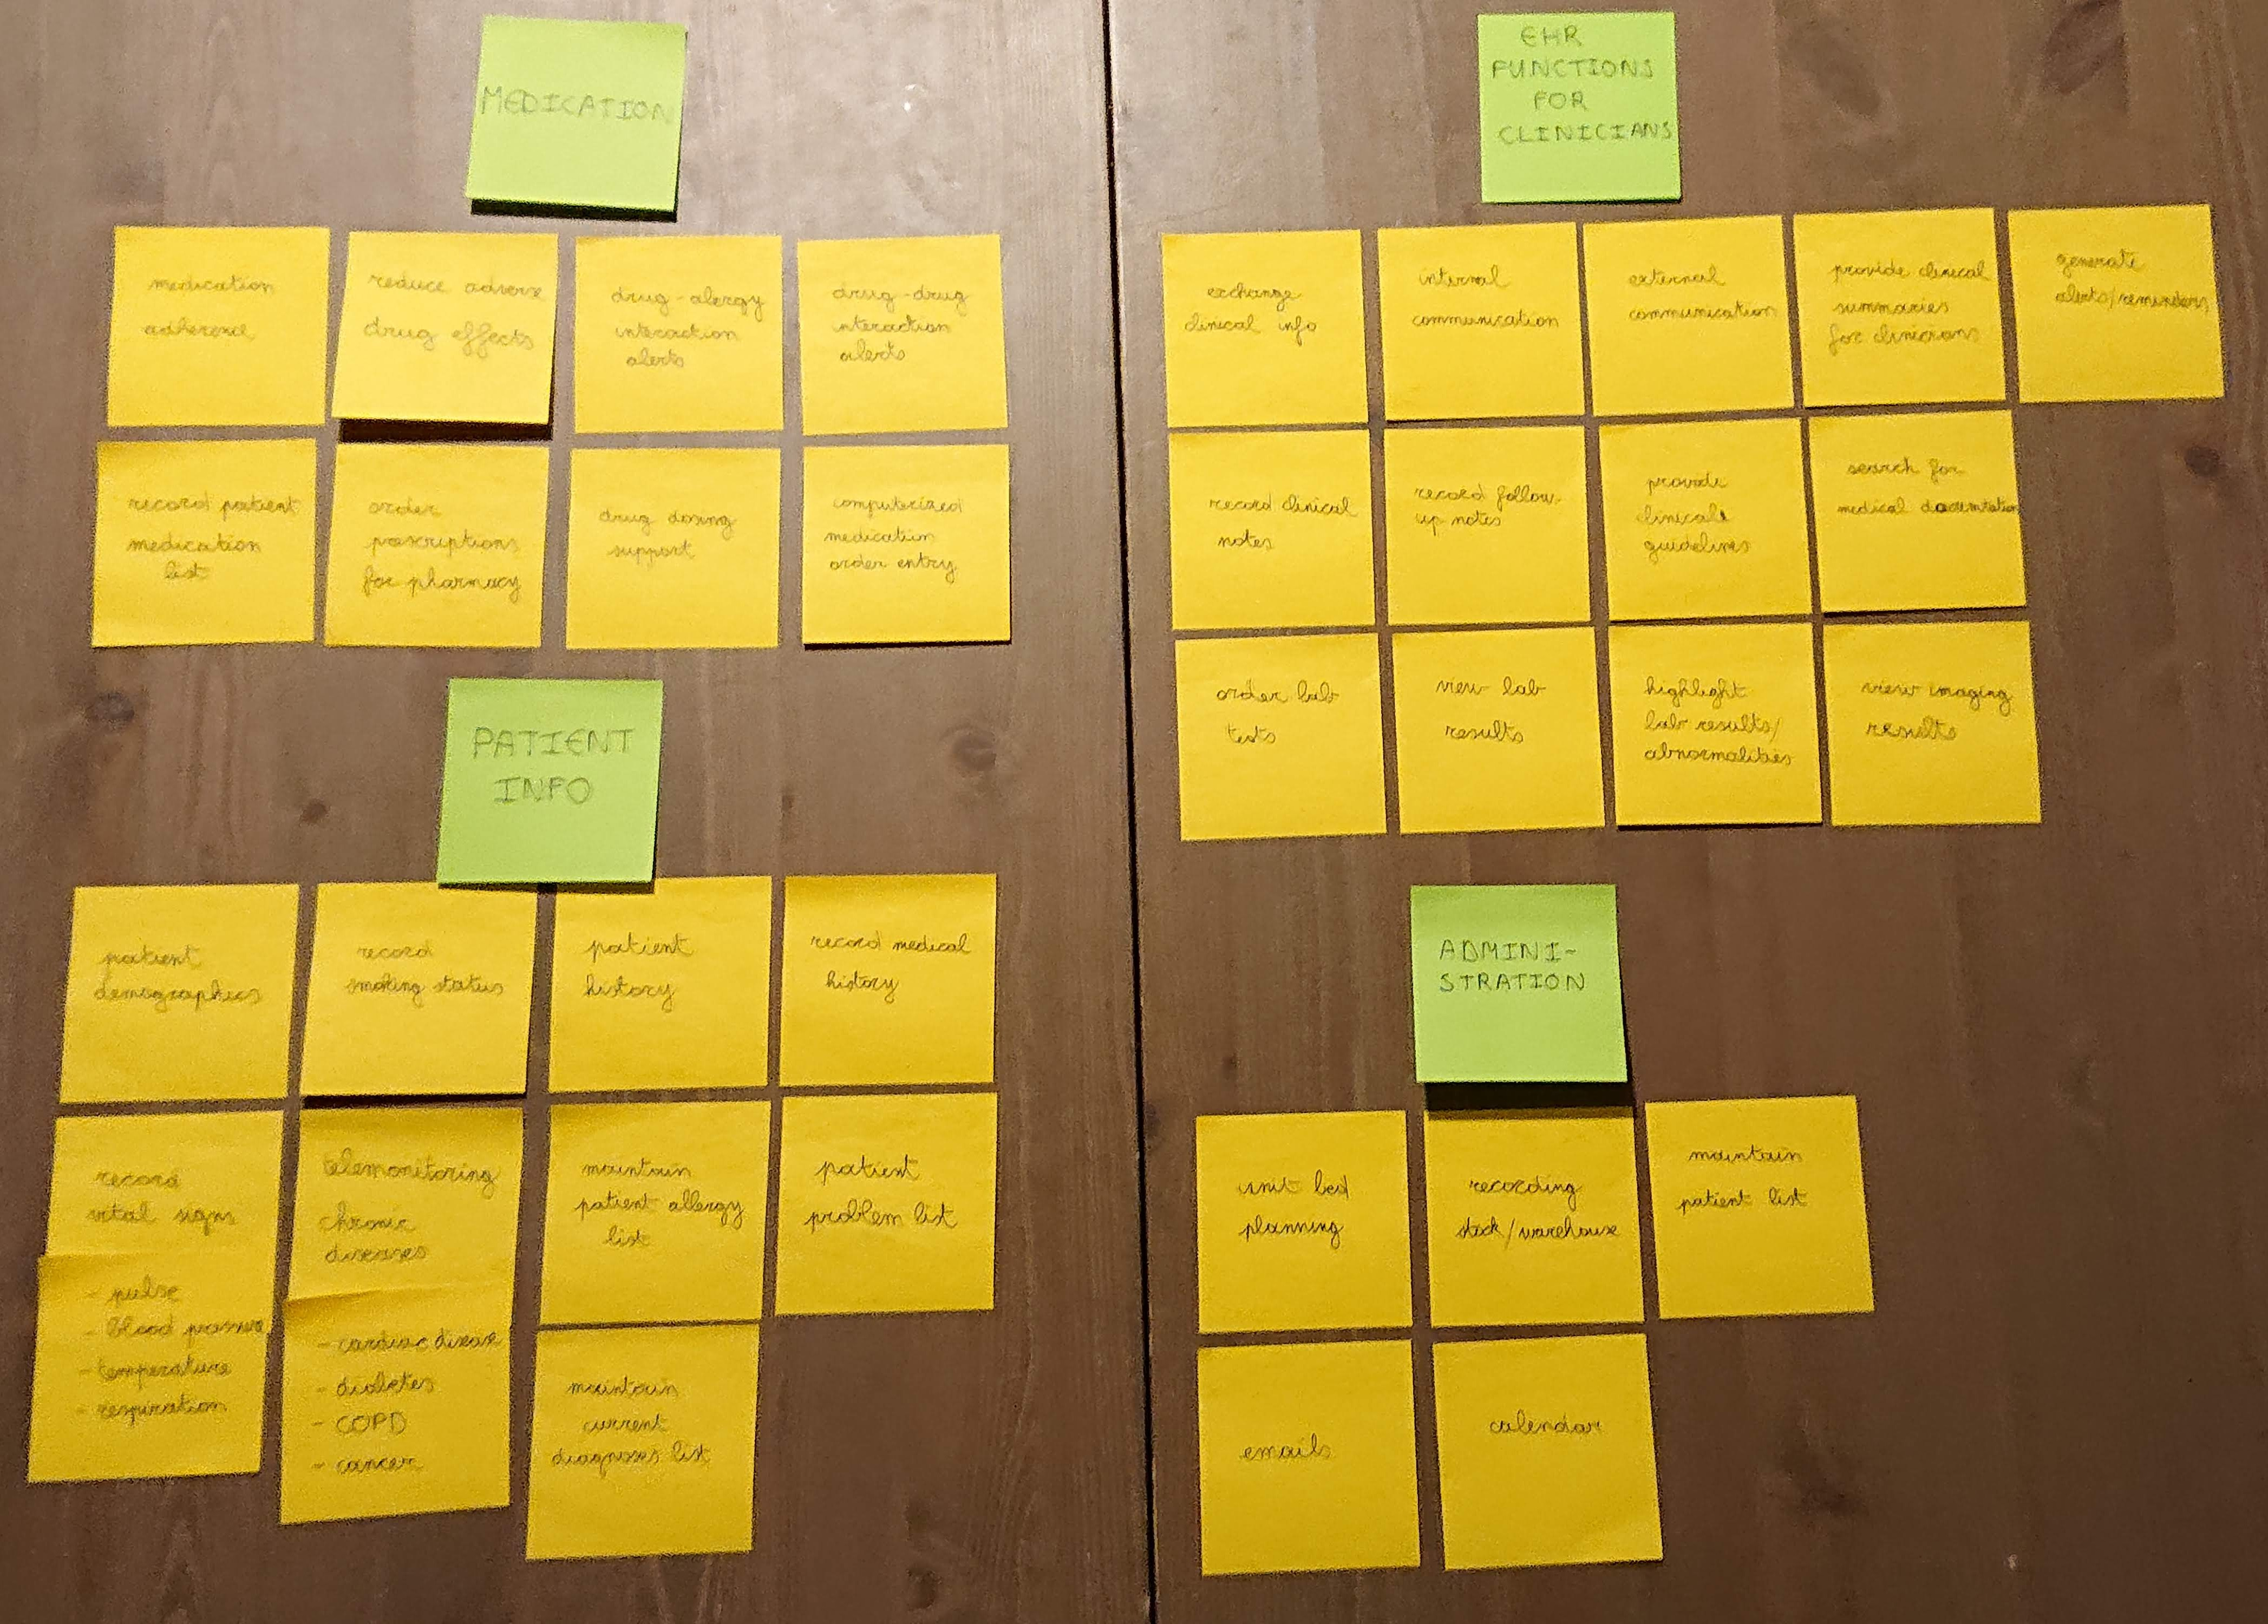
\includegraphics[width=1\textwidth]{chapters/3_design/affinity}
            \caption{The affinity diagram created during the brainstorm session.}\label{fig:affinity}
        \end{figure}
        This section describes the brainstorm session which intends to group the components described in the previous section to form categories. From these categories we pick several modules which we will then implement in our prototype. An ideal tool for this situation are affinity diagrams.

        Affinity diagrams help to categorize and sort a large amount of ideas by grouping similar ideas together and identifying relevant topics~\cite{Affinity}. These diagrams are created by following these five steps:
        \begin{enumerate}
            \item Generate ideas: all components of the lists mentioned the previous section serve as our ideas. Each component was written down on a post-it note. Duplicates between the lists are not skipped because we will get rid of these in later step.
            \item Display the ideas: all post-it notes were placed on a table and shuffled around.
            \item Sort the ideas into related groups: related components were grouped together and duplicates were removed. 
            \item Create header cards for the groups: these are the names of the categories. We found the following categories: medication, patient information, clinician-specific functions, and administration.
            \item Draw the finished affinity diagram: figure~\ref{fig:affinity} displays the result.
        \end{enumerate}

        \paragraph{Result} The following four categories were found:
        \begin{itemize}
            \item \textbf{Medication}: all components related to management of medications and prescriptions. These are: adherence, reduce adverse drug effects, drug-drug interaction alerts, drug-allergy interaction alerts, record patient medication list, order prescriptions for pharmacy, drug dosing support, and computerized medication order entry.
            \item \textbf{Patient information}: components that are related to the management of general patient data. These are: patient demographics, smoking status, patient history, medical history, record vital signs data (pulse, blood pressure, temperature, respiration), telemonitoring (cardiovascular disease, diabetes, COPD, cancer), allergy list, problem list, and a current diagnoses list.
            \item \textbf{Clinician-specific functions}: general components that a clinician uses, but are not related to a patient. These are: exchange clinical information, in- and external communication, view clinical summaries, generate alerts/reminders, record medical and follow-up notes, view medical guidelines, search for medical documentation, order and view lab results, highlight lab result abnormalities, and view imaging results.
            \item \textbf{Administration}: maintain patient list, bed planning, stock and warehouse management, emails, and calendar.
        \end{itemize}

        \noindent Some components such as reminder generation can be applied throughout an EHR system or be implemented as a sub-feature of another component. Literature repeatedly highlighted medication management as an important component of an EHR system, which is also the reason why it is a category. We chose to implement the following modules:
        \begin{itemize}
            \item Patient information: displays demographic information concerning an individual.
            \item Prescription list: create, update, and remove prescriptions, view the current medication scheme of a person, and provide warnings about potential drug interactions.
            \item Allergy list: create, update, and remove allergy entries.
            \item Vaccination list: create, update, and remove vaccination entries.
            \item Workflow: create workflow schedules for a patient. For example, performing checks at certain points in time can be defined here.
            \item History: view the medical history of a patient. This module records all changes made to the medical record of the patient.
            \item Telemonitoring: view data over time for the following parameters: blood pressure, blood sugar, heart rate, blood oxygen level, and weight.
        \end{itemize}

    \subsection{Application specification}\label{app_specification}

    During this section we will describe the different components of the dashboard prototype. This specification should clearly indicate how the application is structured and how it will be used. First we describe the dashboard as a whole, after which we go into more detail for each module.

        \subsubsection{General structure}

        After startup, the user is greeted with a login screen. Once the user successfully authenticated, the patient list is shown. This list shows basic information of all the patients available to the user. It is possible to sort and filter this list. Selecting a patient will open the dashboard and load its corresponding configuration.

        \paragraph{Dashboard} The dashboard consists of two panels. A small panel on the left hand side features the patient information module. Smaller versions of some modules can be added to the panel which each generate a concise summary. Generating a summary is not relevant for every module, which is why some of them will not have smaller counterpart. The smaller modules can only be vertically arranged and resized. Due to the limited size of the left panel, these modules will take up the entire available width. In the case the display of the device is small, the left panel is automatically hidden to give more space to the main panel. Pressing a button in the top left corner will show the summarizing panel on top of the main panel. By supporting smaller screen sizes, the application can be used on mobile devices such as tablets.

        The main panel fills up the remaining width of the display. Modules can be freely placed on this panel. Here, modules can be resized both horizontally and vertically. By providing resize capabilities for the modules, an even larger variety of display screens can be supported. If the screen width changes, then the modules will be rearranged to fit on the new display.

        \paragraph{Layouting} It is possible to create a module layout for each patient. Initially, the dashboard will be empty for all patients. Therefore, the user will need to add modules and arrange them on the dashboard. The layout automatically saves after each change. Dragging modules will push the others aside to give the user a preview of what will happen. Once the module is released, the layout is rearranged.

        \subsubsection{Modules}\label{app_specification_modules}

        We now describe the functionality of each component chosen after the brainstorm session. For each module we describe its goal, functions, and whether it has a small version or not.

        \paragraph{Patient information} This module displays some basic demographic information of the patient. It is always found at the top of the left panel and it can not be removed, because this is information you should always have access to. However, it can be resized to a smaller version to give more space to other modules. We intend to show the following information for each patient: first and last name, gender, date of birth, national identification number, blood type, height, address, phone number, and smoking status. The small version shows only the full name, date of birth, gender, and blood type.

        \paragraph{Prescription list} The prescription list module shows an overview of all the patient's prescriptions during a certain period. The user can create, update, or remove prescriptions. In order to create a prescription, the user has to select a start and end date, a medicine, and the dosage. The dosage can be set for the morning, noon, evening, and bedtime. This is in line with weekly pill boxes that help patients adhere to their medication scheme. Interactions between prescriptions are highlighted if their time periods overlap. When the user clicks on a prescription, the following information regarding the medicine is shown: a description, side effects, and the medicines it interacts with.

        A small version of this module shows the medication scheme of the patient of today. This list only shows the medicine and the dosage. Prescriptions can not be added, updated, or removed from this small version. The sole purpose of this module is to give a summary. As such, the detailed information of the prescriptions are hidden.

        \paragraph{Allergy list} The allergy module presents a list of all the allergies the patient has. This module allows the user to create, update, or remove allergy entries. The following information has to be entered for every allergy: name, description, diagnosis date, allergy type, and the severity. Based on literature, the following allergy types can be chosen: food, skin, respiratory, and drug allergy~\cite{AllergyTypesACAAI, AllergyTypesHealth24}. In case an allergy does not fall within these four types, the user can indicate this. Allergies can be detected via IgE testing. The higher the IgE concentration, the more severe the reaction to the allergy. After consulting literature, five levels of severity can be selected ranging from 1 (mild) to 5 (severe)~\cite{AllergySeverity}. The cited source describes seven levels, with level 0 meaning allergy absence and level 6 meaning extremely severe. These two were omitted as absence to an allergy isn't recorded and level 5 also indicates an extreme severe reaction. This module also has a smaller version, which only shows the severity, name, and type of the allergies.

        \paragraph{Vaccination list} This module is similar to the allergy module, but instead stores vaccination entries. The user can add, update, or remove vaccinations. For each vaccination the disease name and description must be given. Optionally, a date of a future vaccination shot may be entered. Historical vaccinations shots can be added as sub-entries of the vaccination description. These entries contain a description and the date the shot was administered. The smaller version of this module will not show these entries, but only shows the diseases for which the patient is vaccinated and future vaccination data.

        \paragraph{Workflow} Clinicians need to follow certain procedures. The workflow module is a tool to describe these procedures. For example, a patient has received an artificial hip. During the rehabilitation process, the patient has to reach several goals over the next few weeks. A day after the operation, the patient must be able to sit up straight. The patient should be able to stand the next day. These goals can be written down in the workflow module.

        Using this module, users can define workflows and share them if desired. For each new workflow the user must indicate whether it is created specifically for this patient and if the user wants to share the module with other users of the dashboard platform. A workflow consists of a series of steps, which in turn may have sub-steps. Each workflow has a name and a description. The steps of the workflow also have a name and description. However, sub-steps only have a description, as they should be small in scope.

        \paragraph{History} As the user adds, updates, or removes data from the record of the patient, log entries are generated for the history module. It is important to have a historic view of the patient's medical record, which is the primary goal of this module. Each log entry contains information on what changed, what type of operation was executed (create, update, delete), from which module it originated, and the date it happened. The user can filter the history entries to only show certain operations or modules where changes occurred. There is no small module present for this module, because this data is difficult to summarize.

        \paragraph{Telemonitoring} To conclude, the telemonitoring module will provide a visual display of vital signs data. The goal of this module is to help the user to identify trends and to compare data of different parameters with each other. The module will generate a chart on which the data is plotted given the selected time period. The following five parameters can be monitored: blood pressure, blood sugar, heart rate, blood oxygen, and weight. These parameters were chosen since they can be measured from home and are closely related to the four chronic diseases described in~\ref{telemonitoring}.

        The user can choose to plot up to two parameters on the chart, in order to view their data in relation to each other. Comparisons between data from the same parameter, but for different time periods are realized by adding two instances of the module to the dashboard. For example, by placing them next to each other, differences are easily spotted. A small version of this module shows the number of data entries and statistics (lowest, highest, and average value) for the selected parameters from a chosen start date until now.